%!Tex TS-program = xelatex
%!TEX encoding = UTF-8 Unicode

  \documentclass[
  12pt, a4paper,		% tamanho da fonte e papel.
  openright,			% capítulos começam em pág ímpar (insere página vazia caso preciso)
  oneside,			% para impressão em recto somente. Oposto a twoside.
  brazil, english		% o último idioma é o principal do documento, ademais são hifenizados corretamente.
  ]{abntex2}
  \RequireXeTeX %Force XeTeX check

% --- (tudo que vem depois de '%' é um comentário em latex)
% ---
% Pacotes fundamentais 
% ---
\usepackage{lmodern}	% Usa a fonte Latin Modern
\usepackage[T1]{fontenc}% Seleção de codigos de fonte.
\usepackage[utf8]{inputenc}% Codificacao do documento (acentos)
\usepackage{indentfirst}% Indenta o primeiro parágrafo da secção.
\usepackage{color}% Controle das cores
\usepackage{graphicx}	% Inclusão de gráficos
\usepackage{microtype}% para melhorias de
% justificação
\usepackage{xltxtra} %fontspec, metalogo e realscripts (XeLaTex)
\usepackage{lipsum} % Enche linguíça (preenche espaço)
\usepackage[alf]{abntex2cite}% Citações padrão ABNT
\usepackage{amsmath} % Diversas tipografias matemáticas

\begin{document} %% Iniciar o documento

\chapter{Capítulo 1}
\section{Secção número 1.1}

\textbf{De acordo com \cite{knuth1984literate}, Literate programming é o paradigma mais formal e divertido de todos.}

\begin{figure}[ht]
  \centering
  \caption{\label{fig:tower2} Categorization of the study of towers of interpreters}
  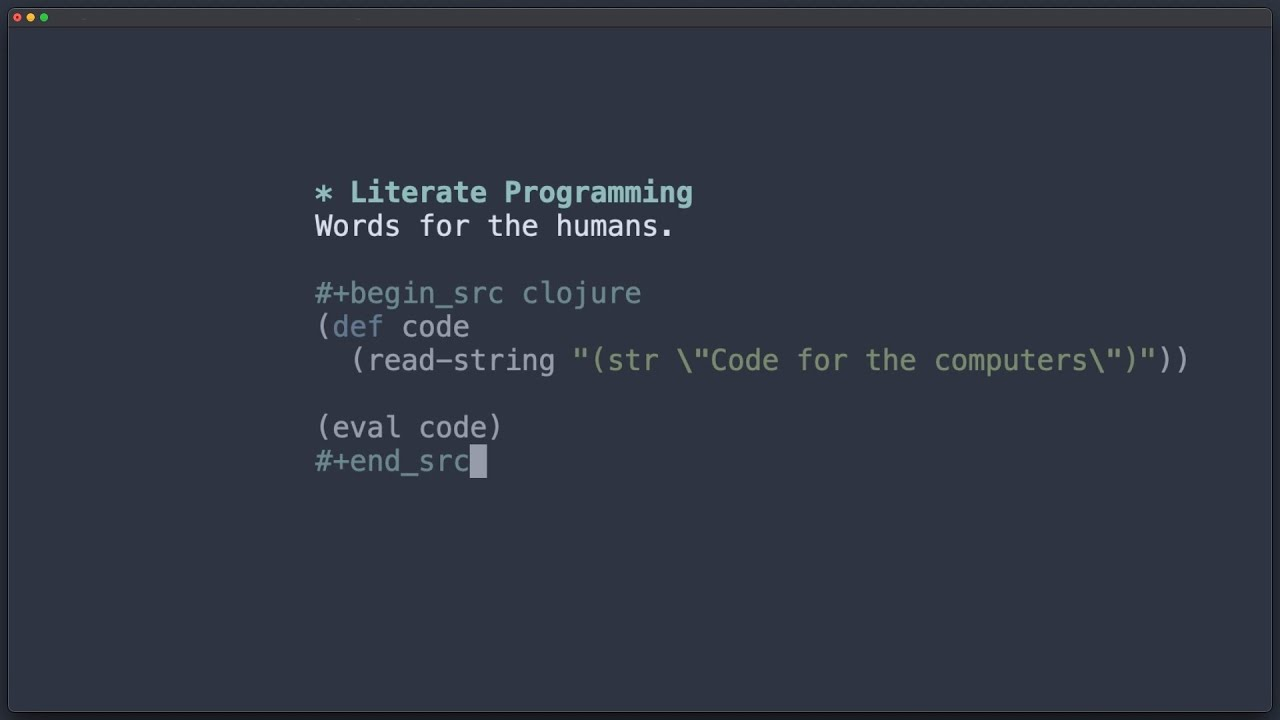
\includegraphics[width=0.5\linewidth]{./img/literate-programming.jpeg}
  \legend{Reference: \cite{amin2017towers}}
\end{figure}

\lipsum[1-2] % Texto enche linguíça

\bibliography{arquivo-com-bibliografias} % Usar bibliografias

\end{document}
